\section{Gatling}

Après mon travail sur \capico{}, j'ai rejoint, avec deux autres stagiaires, Stéphane LANDELLE sur son projet appelé Gatling \cite{gatling} pour le restant de mon stage.

\begin{figure}[H]
 \centering
 
\includegraphics[width=0.3\linewidth]{images/logo_gatling.pdf}
\end{figure}


\subsection{Présentation du projet}

Gatling est une application permettant d'effectuer des tests de charges sur des applications web. Elle a été créée par le directeur technique d'\ebi{}, Stéphane LANDELLE qui en est le responsable. La majeure partie de l'application est open source et disponible sous Apache License v2.0. La partie permettant de générer les rapports utilisant une librairie non open source, est disponible gratuitement mais il est interdit de modifier le code source ou d'utiliser des parties du code en dehors de Gatling.\\

Le fonctionnement de l'application est très simple. L'utilisateur décrit des scénarii de tests dans un fichier à l'aide d'un DSL (Domain-Specific programming Language). Ces scénarii sont une suite de requêtes HTTP à envoyer à l'application web en test pour simuler un utilisateur naviguant dans l'application. Il suffit ensuite de spécifier le nombre d'utilisateurs à simuler. Gatling compile ensuite ce fichier pour exécuter les requêtes et enregistrer dans un journal les valeurs permettant, plus tard, de calculer des statistiques telles que le temps de réponse du serveur.\\

Lorsque tous les scénarii ont été exécutés, Gatling lit le journal, calcul plusieurs statistiques, notamment le temps de réponse du serveur et le nombre de requêtes par secondes, pour générer un rapport sous la forme de pages HTML contenant plusieurs graphiques permettant de réprésenter les résultats.\\

Le fichier décrivant les requêtes à exécuter sont écrits dans un langage de programmation qui n'est pas forcément facile à prendre en main pour tout le monde. C'est pourquoi, Gatling vient avec une application appelée le Gatling Recorder qui permet d'enregistrer les requêtes tout en naviguant sur l'application web avec un navigateur. Le Recorder fonctionne en tant que proxy pour le navigateur. Le scénario de test est donc la simulation de la navigation de l'utlisateur s'enregistrant avec le Recorder.\\

Le projet est lui-même écrit en Scala, un langage de programmation multi-paradigme. Il utilise Akka une librairie Scala/Java permettant de créer des applications concurrentes facilement. Gatling repose sur d'autres librairies telles que Netty ou encore SLF4J.

\begin{figure}[H]
 \centering
 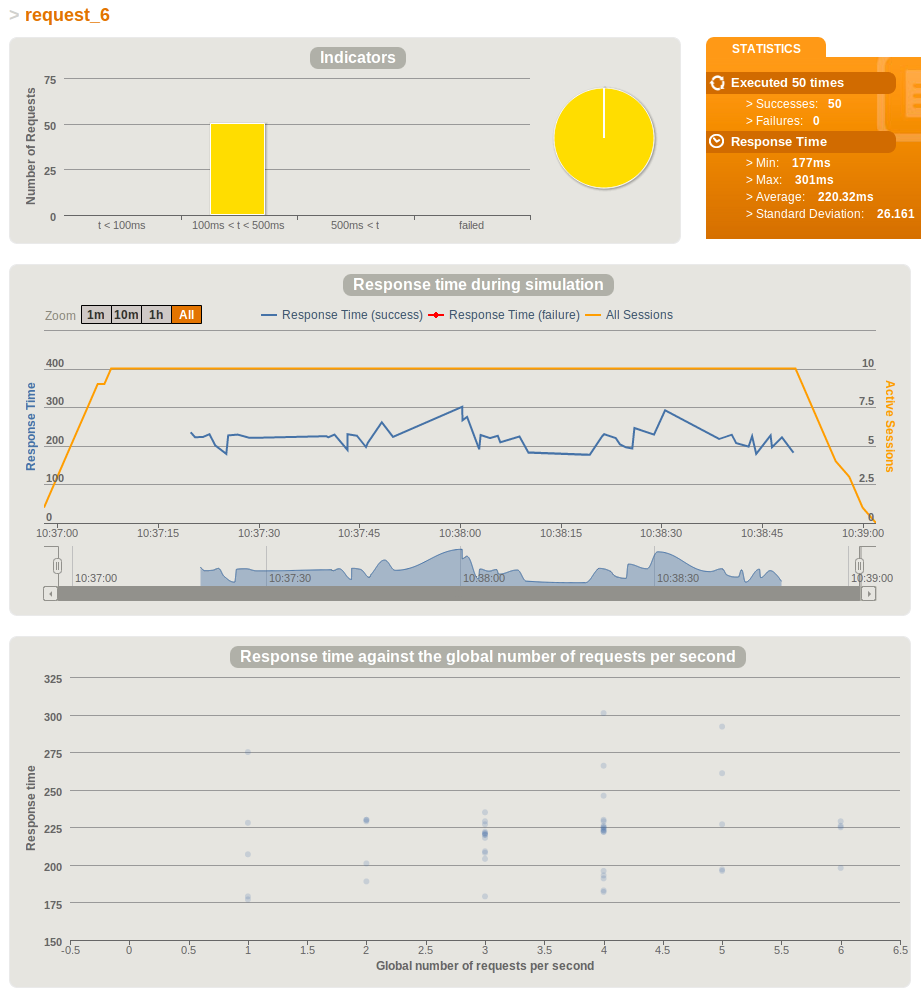
\includegraphics[width=\linewidth]{images/req_details_basic_usage.pdf}
 \caption{Exemple de rapport pour une requête}
\end{figure}

\subsection{Scala}

Gatling est écrit en Scala \cite{scala}, un langage qui mélange les paradigmes de programmation orienté objet et de programmation fonctionnelle. Ce langage a été créé en 2003 par Martin ORDERSKY, qui a aussi travaillé sur \verb+javac+, le compilateur Java. Ce langage qui a presque 10 ans a un sursaut d'engouement depuis l'année dernière avec l'apparition notamment des frameworks Akka et Play qui permettent de créer des applications web directement en Scala.\\

Comme en Java, le code Scala est compilé en bytecode et est exécuté sur une JVM. Scala et Java sont interopérable puisqu'il est possible d'utiliser des API Java en Scala et vice-versa. D'ailleurs, de nombreuses API du SDK Java n'ont pas d'équivalent en Scala, il suffit d'accéder directement à l'API Java.\\

Scala utilise un typage statique des variables, tout comme en Java mais tire beaucoup plus partie de la généricité. C'est à dire le fait de paramétrer une classe ou une fonction par un type. L'objectif étant d'avoir un maximum d'erreur de type découvert par le compilateur et non à l'exécution.\\

Un des avantages de Scala est d'écrire du code beaucoup plus concis qu'en Java, au prix d'une compilation plus lente. Le code Scala est plus concis car une bonne partie de la syntaxe est facultative, notamment grâce à l'inférence de type. Le compilateur est suffisament intelligent pour deviner les parties facultatives.\\

Ce langage permet d'écrire du code vraiment réduit au minimum, ce qui permet de rendre le code plus maintenable. Sa compréhension est cependant plus complexe. De plus, la façon de développer est différente du Java puisqu'on est aussi dans un paradigme de programmation fonctionnelle.\\

Il a donc nécessité un temps d'adaptation avant de pouvoir comprendre le fonctionnement interne de Gatling et de pouvoir développer de nouvelles fonctionnalités.

\subsection{Akka}

Akka \cite{akka} un framework avec une API Scala et une API Java pour faire des applications concurrentes. Le framework Akka permet de s'abstraire des threads qui sont utilisés pour pouvoir exécuter des parties du code en parallèle. Dans le cas de Gatling, l'objectif est d'envoyer plusieurs et surtout beaucoup de requêtes en parallèle.\\

Akka s'abstrait des threads en introduisant les acteurs. Les acteurs sont des entités qui s'exécutent en parallèle. Un acteur possède une boite aux lettres qui permet de recevoir des messages. L'exécution d'un acteur est démarré par la réception d'un message.\\

En interne, Akka utilise un pool de threads pour exécuter les acteurs. Akka permet d'avoir potentiellement un très grand nombre d'acteurs qui s'exécutent (plus de 1000) sur un pool de threads restreints. Le problème lorsqu'on développe une application concurrente c'est la performance. En effet, plus on veut exécuter de tâches en parallèle, plus on créé de threads. Cependant, lorsque trop de threads sont créés, les performance sont diminuées. Akka permet de répondre à ce problème puisqu'il utilise un nombre restreints de threads.

\subsection{Récupération des métriques serveurs}

La première fonctionnalité sur laquelle nous avons effectué des recherches est la récupération des métriques serveurs. En effet, actuellement seules les métriques côté client sont enregistrées comme par exemple le temps de réponse ou le nombre de requêtes par secondes. L'objectif est donc de récupérer les statistiques du serveur telles que la charge du serveur ou l'état de la mémoire pour pouvoir mettre en relation les métriques serveurs avec les métriques clientes.\\

Pour pouvoir mettre en place cette fonctionnalité, nous avons donc recherché les technologies à utiliser, puis nous les avons testé et surtout vérifié leur impact sur les performances.\\

\subsubsection{Java Management eXtensions}

La première technologie que nous avons trouvé est Java Management eXtensions (JMX) \cite{jmx}. JMX est une API Java qui permet de gérer à distance des applications s'exécutant sur une JVM. Elle permet de récupérer des informations exposées par JMX telles que l'utilisation du CPU par la JVM, mais elle permet aussi d'appeler des méthodes distantes pour par exemple redémarrer des composants.\\

En interne, JMX repose sur RMI (Remote Method Invocation), une API Java qui permet d'appeler des méthodes sur des objets distants. L'utilisation de JMX est extrêmement simple, puisqu'il suffit de créer une interface dont le nom se termine par \verb+MBean+ ainsi qu'une classe implémentant cette interface. Elle sera alors automatiquement exposée par JMX et accessible de l'extérieur.\\

Pour pouvoir facilement accéder aux objets exposés (appelés MBean), nous avons utilisé JVisualVM, un programme fournit avec le JDK (Java Development Kit) d'Oracle. Ce programme permet de monitorer des JVM locales ou distantes en accédant notamment aux MBean.

\begin{figure}[H]
 \centering
 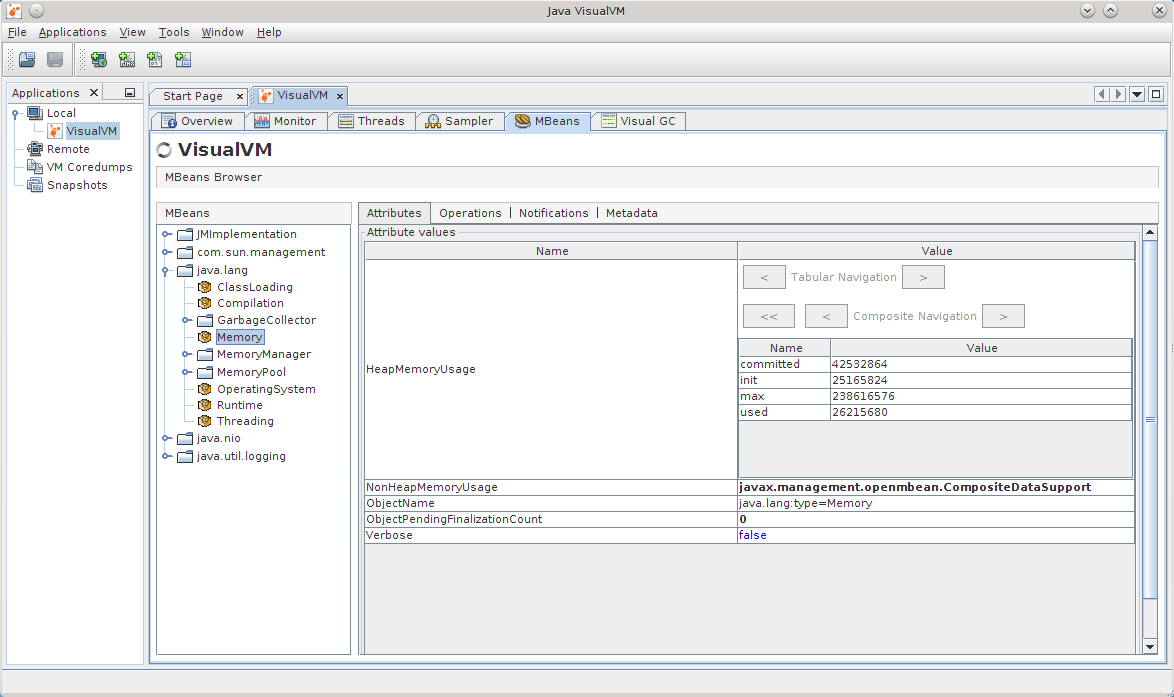
\includegraphics[width=\linewidth]{images/jvisualvm.pdf}
 \caption{Utilisation de JVisualVM pour accéder aux MBean}
\end{figure}


L'utilisation de JMX est donc très simple, de plus, plusieurs métriques sont déjà exposées par la JVM, telle que l'utilisation du CPU, l'utilisation de la Heap (mémore interne de la JVM), la durée totale de collection par le Garbage Collector (GC), \dots{}\\

Cependant, un des inconvénients de l'utilisation de JMX est l'utilisation sous-jacente de RMI qui déclenche régulièrement le GC. L'exécution du Garbage Collector étant coûteuse en performance, son utilisation peut avoir un impact. En effet, nous voulons utiliser JMX pour récupérer des informations sur le serveur qui est en train d'être testé. L'utilisation de JMX peut donc interférer avec les performances du serveur et fausser les résultats du test de charge.

\subsubsection{Agent Java}

La deuxième technologie est l'utilisation d'un agent java. Un agent java est un code Java qui est exécuté au démarrage de la JVM avant la méthode \verb+main+. Un agent permet notamment de manipuler le bytecode d'une classe au chargement de celle-ci. On peut aussi utiliser un agent pour exécuter du code en parallèle de l'application et donc par exemple, écrire dans un fichier les métriques que l'on veut récupérer.\\

Un des inconvénients des agents est qu'il faut modifier la ligne de commande qui démarre le serveur pour pouvoir ajouter notre agent. Son utilisation est donc assez complexe puisqu'il nécessite une intervention de la personne qui souhaite utiliser Gatling.\\

Cependant, Sun a créé une API permettant d'attacher un agent à une JVM déjà en cours d'exécution. Il est donc possible d'attacher notre code à une JVM de façon assez simple. Cette API possède une limitation puisqu'on ne peut attacher un agent uniquement à une JVM locale et non distante. Son utilisation nécessite donc toujours une intervention de l'utilisateur de Gatling, mais l'intervention est plus simple puisqu'il ne s'agit que d'exécuter un programme qui va découvrir les JVM et attacher l'agent.\\

Un agent permet donc d'exécuter notre code et donc de créer des sondes qui vont permettre d'enregistrer ou d'envoyer à une application tierce, les métriques que l'on souhaite récupérer. Ces sondes peuvent bien évidemment tirer partie de JMX pour exposer les métriques.

\subsubsection{Sigar}

Nous nous sommes ensuite renseigné sur des API permettant de récupérer des informations de la machine elle-même. Cette partie est plus complexe puisqu'elle est dépendante du système d'exploitation. Nous avons alors trouvé Sigar développé par Hyperic \cite{sigar}.\\

Sigar répond tout à fait à la problématique pusqu'il propose une API indépendante du système d'exploitation mais fonctionnant à la fois sur Windows, Mac OS X, Linux, \dots{} Il utilise JNI (Java Native Interface) pour faire appel à des librairies écrites en C dépendantes, elles, du système d'exploitation.\\

Son utilisation assez simple a un inconvénient : la librairie correspondante au système d'exploitation doit être accessible par le code qui utilise Sigar. Il faut donc que l'utilisateur de Gatling installe Sigar sur le système contenant le serveur.\\

Cependant, si on considère l'utilisation de Sigar avec un agent, il suffit de mettre dans l'archive contenant l'agent, toutes les librairies pouvant être utilisées. Son utilisation est donc envisageable.

\subsubsection{Metrics}

Le dernier point sur lequel nous avons fait des recherches est sur la façon d'enregistrer les métriques du serveur. À la fin de l'exécution du test de charge, les métriques doivent être mises à disposition de Gatling, c'est la seule contrainte.\\

Nous avons donc envisager plusieurs solutions :

\begin{itemize}
 \item Écrire dans un fichier puis l'envoyer à Gatling à la fin du test,
 \item Écrire dans une base de donnée SQL ou NoSQL distante,
 \item Envoyer les données au fur et à mesure à Gatling.\\
\end{itemize}

Les deux dernières solutions consomment de la bande passante ce qui est un sérieux inconvénient puisque le trafic vers le serveur est sûrement surchargé à cause du test. La première solution, quand à elle, risque d'impacter les performances côté serveur à cause des accès disques.\\

Nous nous sommes alors rendu compte que ces solutions pouvait dépendre du cas d'utilisation et qu'il était plus intelligent de laisser le choix à l'utilisateur de Gatling. Il nous fallait donc un système qui permette de s'abstraire de la méthode d'enregistrement des résultats. Pour cela, nous avons décidé d'utiliser Metrics \cite{metrics}, développé par Yammer, un système social privé pour entreprise.\\

Metrics permet de consolider des données sous forme de statistiques, c'est à dire sous la forme d'une simple valeur, d'un compteur, d'un histogramme, \dots{} Metrics permet aussi d'envoyer régulièrement ces statistiques vers différents systèmes : un fichier, des applications de monitoring tierces (Graphite, Ganglia), via JMX \dots{}\\

Avec Metrics, il est aussi possible de créer notre propre système d'écriture des données pour envoyer les statistiques vers une base de données par exemple.

\subsubsection{Notre solution}

La solution que nous avons conçut mais pas développé est la suivante : nous utilisons un agent que nous attachons au serveur via l'API Attach. Cet agent accède aux informations de la JVM via JMX en local et aux informations de la machine via Sigar. Les données sont consolidées par Metrics et enregistrées via un système configurable : écriture dans un fichier ou dans une base de données.\\

Nous n'avons pas développé cette solution pour plusieurs raisons :
\begin{itemize}
 \item Elle impact les performances du serveur en test et fausse donc les résultats,
 \item Notre problématique se rapproche beaucoup du monitoring d'un serveur pour lequel il existe des solutions déjà toutes faites.\\
\end{itemize}

Cette fonctionnalité n'avait donc pas vraiment sa place dans Gatling.

\subsection{Exposition des métriques Gatling}

Si la précédente fonctionnalité n'a pas été développée, elle a donné l'idée d'exposer les statistiques de Gatling pour être accessibles à un système tiers. En effet, pour le monitoring de serveur, des applications telles que Graphite et Ganglia sont très utilisées. L'objectif était donc d'envoyer les mesures faites par Gatling vers ces systèmes.\\

Pour mettre en place cette fonctionnalité, il a simplement fallu utilisé Metrics, qui permet déjà d'exposer les métriques via JMX mais aussi d'envoyer ces informations vers Graphite et Ganglia. L'activation de cette fonctionnalité est faite via le fichier de configuration.\\

Je n'ai que très peu travailler sur cette fonctionnalité, donc je ne m'étendrai pas dessus. Mon travail s'est restreint a tester Metrics en faisant un mini-projet pour vérifier son utilisabilité.

\subsection{Génération du rapport}

Je suis ensuite passé sur une troisième fonctionnalité pour le restant de mon stage. Cette fonctionnalité est une amélioration d'une partie de Gatling et est due à une remarque d'un utilisateur. Cet utilisateur a testé son application pendant 48 heures générant un journal de 8 Go à traiter pour créer le rapport. Cependant cette génération du rapport chargeait le fichier en mémoire, ce qui demande une machine possédant une importante quantité de mémoire.\\

Pour mieux comprendre, voici le fonctionnement de Gatling :
\begin{enumerate}
 \item Compilation du scénario de test,
 \item Exécution des requêtes du scénario. Chaque exécution génère une ligne dans le journal contenant des informations brutes telles que le succès ou l'échec de la requête, le nom de la requête, l'heure de début et de fin de la requête, l'heure de début et de fin de la réponse,
 \item Lorsque le scénario est fini, le journal est traité pour généré le rapport final.\\
\end{enumerate}

Il y a plusieurs avantage à cette méthode :
\begin{itemize}
 \item Il n'y a pas de perte de performances due au calcul de statistiques pendant le test,
 \item Si Gatling plante, peu importe la raison, les données ne sont pas perdues car écrites au fur et à mesure. Il est possible alors de relancer Gatling uniquement pour générer le rapport.\\
\end{itemize}

La génération du rapport utilisée auparavant chargeait tout le fichier en mémoire pour pouvoir le traiter. En effet, c'est la méthode la plus simple pour pouvoir déterminer des statistiques telles que les quantiles (médiane, 95\ieme{} percentile, 99\ieme{} percentile).\\

Nous nous sommes donc renseigné sur les systèmes permettant de traiter des quantités importantes de données sans impacter de façon significative la mémoire utilisée.

\subsubsection{MapReduce}

Popularisé par Google, MapReduce est un modèle de programmation permettant de traiter de façon parallèle et distribué une quantité importante de données (plusieurs téraoctets). MapReduce modélise la chaîne de traitement des données par une succession de tâches \verb+map+ et \verb+reduce+.\\

Une tâche \verb+map+ correspond à un traitement donnée par donnée. Voici la signature en pseudo-code de la fonction \verb+map+ :

\begin{center}
 \verb+map(key: K1, value: V1): (K2, V2)+
\end{center}

Cette fonction permet donc d'appliquer un traitement à chaque paire clé/valeur pour renvoyer une paire clé/valeur. Les types ne sont pas forcément identiques. La tâche \verb+reduce+ permet à partir d'un ensemble de données de calculer un résultat unique :

\begin{center}
 \verb+reduce(key: K, values: List<V1>): V2+
\end{center}

Une telle fonction permet de regrouper toutes les valeurs dont la clé est identique et de calculer un résultat unique.\\

L'idée de MapReduce est de ne simplement écrire que les tâches \verb+map+, \verb+reduce+ et leur enchaînement. Le système s'occupe de diviser les données en entrée en petites unités, exécuter les différentes tâches en parallèle et distribué sur ces unités, regrouper les données pour les tâches \verb+reduce+, \dots{}\\

Cette méthode de calcul n'étant qu'une méthode, nous avons cherché comment la mettre en place pour voir si elle est utilisable dans notre cas.

\subsubsection{Apache Hadoop}

Une des implémentations open source de MapReduce est le projet Apache Hadoop \cite{hadoop}. Il propose une API simple pour créer les tâches puisqu'il suffit simplement d'implémenter les interfaces Mapper et Reducer. Hadoop repose sur un système de fichier distribué appelé HDFS pour pouvoir s'exécuter en parallèle dans un cluster de machines.\\

De toute évidence, nous ne cherchions pas a effectuer des calculs distribués, nous nous sommes donc pencher sur une utilisation simpliste de Hadoop en local. Mais nous avons trouvé que l'écriture de tâches \verb+map+ et \verb+reduce+ est assez complexe et surtout très verbeuse car bas niveau.\\

Nous avons donc cherché des librairies d'abstraction à Hadoop pour nous simplifier le travail.

\subsubsection{Cascading et Scalding}

Il existe plusieurs librairies d'abstraction, certaines plus abouties que d'autres. Celle que nous avons retenue s'appelle Cascading. Elle permet d'écrire un traitement de plus haut niveau avec des fonctionnalités telles que le GroupBy au sens SQL, \dots{}\\

Un autre avantage à Cascading est son mode local qui ne s'appuie pas sur Hadoop mais sur une implémentation intelligente en mémoire dont l'objectif est de tester les traitements en Cascading. Bien qu'a des fins de tests, il faut se pencher sur l'ordre de grandeur de la quantité de données à traiter. MapReduce traite des téraoctets de données. On peut donc supposer qu'un framework de test traite des données en quantités plus faibles, mais de quel ordre ? Gigaoctets ? Mégaoctets ? Nous avons donc voulu tester ses capacités et comprendre comment cela fonctionnait.\\

Après ces tests, nous avons pu comprendre les limites de ce mode local. La limite principale n'est pas tellement la taille du fichier en entrée mais le nombre de données intermédiaires. En effet, le mode local est suffisamment intelligent pour exécuter un maximum de calcul au fur et à mesure de la lecture du fichier. Le seul traitement bloquant étant un \verb+reduce+ qui a besoin de toutes les données pour avoir le résultat. Cependant, un \verb+reduce+ n'a pas besoin de toutes les données en mémoire pour s'exécuter, les calculs peuvent passer par des résultats partiels.\\

Pour mieux comprendre son fonctionnement, voici un exemple de traitement :
\begin{figure}[H]
	\centering
	\includegraphics[width=0.7\textwidth]{images/cascading.pdf}
\end{figure}

Ce traitement est simple : pour chaque ligne, on calcul la différence entre \verb+c+ et \verb+b+, puis on regroupe par \verb+a+. Pour chaque groupe, on calcul le moyenne de \verb+d+. Avec le mode local de Cascading, ce calcul s'effectue en une étape : à chaque ligne, on applique la tâche \verb+map+, puis on calcul le résultat partiel pour la tâche \verb+reduce+. Voici le schéma pour mieux comprendre :

\begin{figure}[H]
	\centering
	\includegraphics[width=0.7\textwidth]{images/cascading_real.pdf}
\end{figure}

Ainsi tout le fichier n'est pas en mémoire. Bien sur, pour que dans notre exemple le résultat soit juste pour plus de données, il faut avoir le nombre de données nécessaires pour calculer un résultat partiel pour pouvoir calculer le suivant. Cette donnée intermédiaire n'est pas représentée mais est bien présente.\\

Cascading va donc fusionner les tâches \verb+map+ entre chaque tâche \verb+reduce+ et calculer cette dernière au fur et à mesure. Les résultats en mémoire ne seront donc que les résultats des \verb+reduce+ intermédiaires. Il y a bien sur des cas où il faut toutes les données en mémoires : la fonction utilisée pour le \verb+reduce+ n'est pas associative, c'est à dire que l'ordre d'application pour réduire une liste de données à un résultat dépend de l'ordre des données en entrées.\\

De plus, dans la mesure ou les résultats des \verb+reduce+ intermédiaires est en mémoire, il faut qu'ils puissent tenir en mémoire. Le comportement du mode local de Cascading dépend donc des calculs. Dans notre cas, la librairie utilisée pour afficher les résultats n'affiche pas plus de 5000 points par courbe, par graphique. La première étape du calcul est donc de regrouper les données par nom de la requête, status de la requête (succès ou échec) et par classe. La classe étant calculée de façon qu'il n'y ait pas plus de 5000 classes. La nature de nos calculs fait que peu importe la taille du fichier en entrée les résultats intermédiaires ont une empreinte mémoire très faible (moins de 200 Mo pour un test de 48h).\\

Après avoir compris que le mode local de Cascading était utilisable dans notre cas, nous nous sommes renseigné comment l'utiliser de façon simple en Scala. Nous avons alors trouvé Scalding, une abstraction à Cascading en Scala, dont le fonctionnement mimique celui des collections en Scala.

\subsubsection{Développement de l'amélioration}

Pour mettre en place l'amélioration, nous avons commencé par développer une application standalone qui permette de générer le rapport à partir du journal. Cette application effectue un traitement en 3 phases :

\begin{enumerate}
 \item Lecture complète du fichier en Scala pur pour déterminer des valeurs générales nécessaires au traitement, notamment l'heure de début et l'heure de fin du test. Ces deux valeurs vont permettre de déterminer les classes pour ne garder que 5000 valeurs au plus pour les statistiques telles que le nombre de requêtes par classes au cours du test.
 \item Traitement avec Scalding utilisant Cascading en mode local, ce qui permet de calculer la quasi-totalité des statistiques.
 \item Calcul des dernières statistiques notamment les quantiles et le nombre de sessions actives par classe au cours du test. Ces calculs nécessitent de parcourir une liste de valeur dans un ordre précis avec une connaissance de la précédente valeur, ce qui n'est pas possible en MapReduce. Ainsi, la distribution des valeurs est déterminée par l'étape 2 mais les quantiles à cette étape. De même, pour les sessions actives, l'étape 2 détermine le nombre de sessions actives en plus ou en moins par classe. Cette 3\ieme{} étape fait l'accumulation des données pour avoir le nombre de sessions actives par classe.\\
\end{enumerate}

Une fois l'ensemble des statistiques calculées avec notre méthode, nous l'avons testée avec un journal de 8 Go. Le résultat s'est calculé en 14 minutes avec une empreinte mémoire de moins de 200 Mo. L'empreinte mémoire a été déterminée avec JVisualVM qui permet d'afficher l'utilisation de la mémoire d'une JVM en cours d'exécution. Les 14 minutes correspondent au temps nécessaire pour lire le fichier 2 fois. Les calculs étant plus rapide que la lecture sur disque, il est donc normal que la partie bloquante soit la lecture.\\

Nous avons ensuite intégré notre travail dans Gatling, en remplaçant l'implémentation actuelle de la génération du rapport par la notre. Bien que celui-ci soit intégré, il est pour l'instant dans une branche de test pour vérifier que tout fonctionne bien et que les résultats sont justes. Lorsque cette méthode aura été suffisamment testée, l'amélioration sera intégrée dans la branche principale de développement du projet.

\subsubsection{Conclusion}

L'utilisation de Cascading en mode local, nous aura permis de comprendre la nécessité de tester les frameworks que l'on pourrait utiliser. En effet, notre utilisation de Cascading en production n'est pas recommandée car nous utilisons une partie qui normalement sert de test. C'est cependant à mettre en perspective par rapport à l'utilisation en production : Cascading sert à traiter des téraoctets de données. La volumétrie est donc importante ici puisque dans notre cas nous ne traitons que des journaux de quelques gigaoctets au maximum.\\

Scalding s'est avéré être très utile car l'écriture du traitement est beaucoup moins verbeuse et plus intuitive qu'en Cascading, cependant, cette librarie créée par Twitter est très mal conçue car elle dépend fortement de Hadoop, même si on utilise le mode local de Cascading. On est donc obligé d'avoir une dépendance à Hadoop bien que nous ne l'utilisons pas.
